
Machine learning is the field of computer science where the computer uses a set of algorithms to learn properties from a given data set $\mathcal X$. The first machine learning problems involved learning a function $f: \mathcal X \to \mathcal Y$ that mapped an input $x \in \mathcal X$ to a label $y \in \mathcal Y$. This discipline is commonly known as \emph{Supervised Learning}.

As years passed, diverse algorithms that manage to find truly complex $f$ functions have been developed and new problems have emerged. Supervised learning has a huge cost: all the examples in the dataset must be labeled. The coss of this resided in the fact that labeling examples is a slow process, and has to be done mostly manually. 

\emph{Unsupervised learning} avoids this problem by trying to infer properties of de data using the \emph{unlabeled} dataset. By not needing to have the labels of our examples, companies can save money and time that they would have invested creating a tag for each example.

When the dimension of the data is high, for instance when treating images computationally, it is usual to first create a \emph{representation} of the input data. Combining this idea with unsupervised learning, we reach to the field of \emph{representation learning}, which studies how to create representations of the data that are useful for performing other tasks such as classification.

Ideally, we would like the original data and the representation created to contain the same information. A way of measuring this is using the \emph{mutual information} $I(X,Z)$ between the input $X$ and the representation $Z$. The mutual information is expressed as:
\[
I(X,Z) = H(X) - H(X|Z),
\]
where $H(X)$ is the entropy of $X$ and $H(X|Z)$ is the conditional entropy.

\begin{figure}[H]
    \centering
    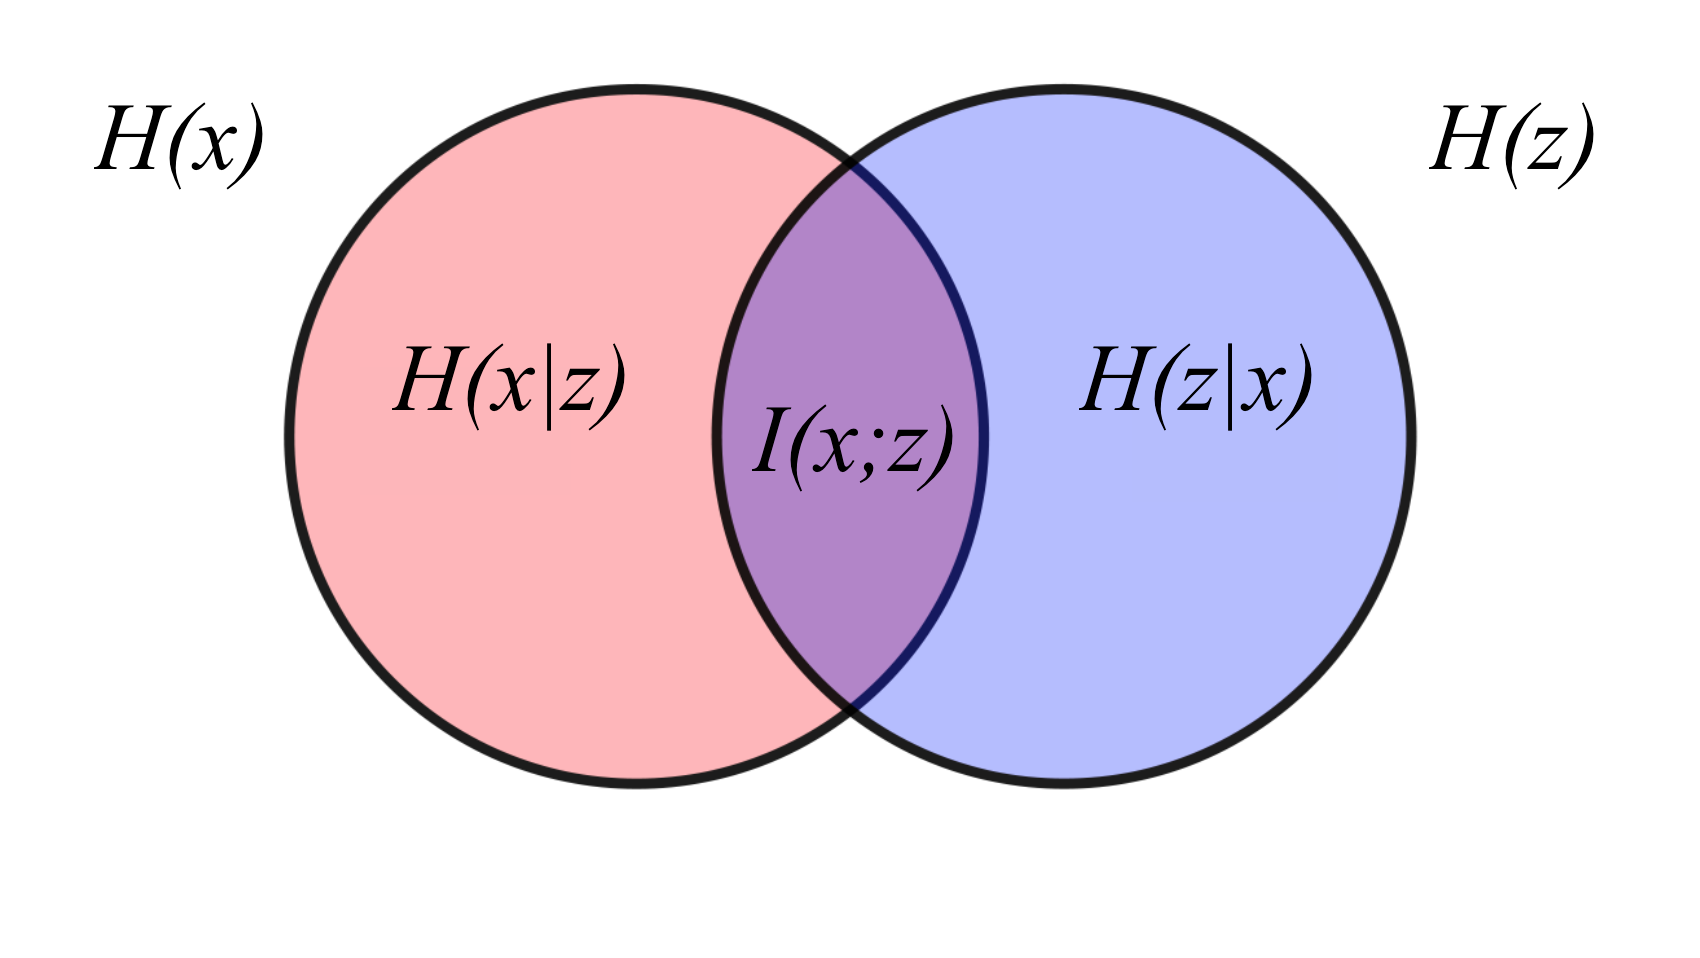
\includegraphics[scale=0.3]{mutual-info}
    \caption{Venn Diagram showing the relationships between the entropies and the conditional entropies of random variables $X$ and $Z$.}
\end{figure}

Since the entropy is a way of measuring ``\emph{how surprising is that an event occurs}'', intuitively the mutual information measures the decrease of uncertainty that we obtain in $X$ when we know that $Z$ has occurred.

Calculating the mutual information between two variables, however, is not an computationally easy problem. Because of this, a way to approach the mutual information maximization is by obtaining lower bounds and maximizing them. Although a few more bounds are proved in this document, we remark the \emph{Contrastive Lower Bound} on the mutual information, which is expressed as follows:
\[
I(X,Z)  \geq - \ell(\theta) + \log N.
\]
In this equation, $\ell(\theta)$ refers to the contrastive loss, which happens to be crucial in representation learning. In short, the \emph{contrastive learning} problem consists in considering elements obtained from the same distribution and elements obtained from a different distribution and learning how to discriminate between the elements of the different distributions. In order to do this, the recently mentioned contrastive loss is used, which usually takes the form
\[
\mathcal L_N = - E_X \left[ \log \frac{f(x,z)}{\sum_{x_j \in X}f(x_j,z)}\right].
\]  
The use of this contrastive loss maximizing the mutual information had a huge impact on the state of art results of representation learning in 2018, achieving very promising results.

However, during the development of this work, this drastically changed. New papers appeared stating that the success of the methods that were maximizing mutual information between the input and its representation was not caused by mutual information, but by the specific form that the contrastive loss has.